\documentclass{article}

\usepackage[utf8]{inputenc}
\usepackage{amsthm}
\usepackage{amssymb}
\usepackage{mathtools}
\usepackage{graphicx}
\usepackage{mdframed}
\usepackage{float}
\usepackage[top=0.75in, bottom=0.75in, left=0.75in, right=0.75in]{geometry}
\usepackage{gauss}

\usepackage{array}
\allowdisplaybreaks

\makeatletter
\newcounter{elimination@steps}
\newcolumntype{R}[1]{>{\raggedleft\arraybackslash$}p{#1}<{$}}
\def\elimination@num@rights{}
\def\elimination@num@variables{}
\def\elimination@col@width{}
\newenvironment{elimination}[4][0]
{
    \setcounter{elimination@steps}{0}
    \def\elimination@num@rights{#1}
    \def\elimination@num@variables{#2}
    \def\elimination@col@width{#3}
    \renewcommand{\arraystretch}{#4}
    \start@align\@ne\st@rredtrue\m@ne
}
{
    \endalign
    \ignorespacesafterend
}
\newcommand{\step}[2]
{
    \ifnum\value{elimination@steps}>0\sim\quad\fi
    \left[
        \ifnum\elimination@num@rights>0
            \begin{array}
            {@{}*{\elimination@num@variables}{R{\elimination@col@width}}
            |@{}*{\elimination@num@rights}{R{\elimination@col@width}}}
        \else
            \begin{array}
            {@{}*{\elimination@num@variables}{R{\elimination@col@width}}}
        \fi
            #1
        \end{array}
    \right]
    & 
    \begin{array}{l}
        #2
    \end{array}
    \addtocounter{elimination@steps}{1}
}
\makeatother

\DeclarePairedDelimiter{\abs}{\lvert}{\rvert}
\DeclarePairedDelimiter{\norm}{\lvert \lvert}{\rvert \rvert}

\newtheoremstyle{break}% name
  {}%         Space above, empty = `usual value'
  {}%         Space below
  {\itshape}% Body font
  {}%         Indent amount (empty = no indent, \parindent = para indent)
  {\bfseries}% Thm head font
  {.}%        Punctuation after thm head
  {\newline}% Space after thm head: \newline = linebreak
  {}%         Thm head spec

\newtheorem{Def}{Definition}[section]

\theoremstyle{break}

\newtheorem{innerEx}{Exempel}[section]
\newtheorem{sats}{Sats}[section]
\newtheorem{Rem}{Anmärkning}[]

\newenvironment{Ex}
{\begin{mdframed} \begin{innerEx} \vspace{3pt}}
{\vspace{3pt} \end{innerEx} \end{mdframed}}  

\newenvironment{bevis}
{\begin{mdframed} \begin{proof} \vspace{3pt}}
{\vspace{3pt} \end{proof} \end{mdframed}}


\title{
	 Linjär Algebra\\
	 Föreläsning 19
    \author{Erik Sjöström}
}
\begin{document}
\maketitle

\section{Sökalgoritmer?} % (fold)
\label{sec:_}

Man tänker sig internet som en riktad graf där noden $v_i$ är en webbsida och kanten $(v_i, v_j)$ är länk från webbsida $v_i$ till $v_j$.

\begin{center}
	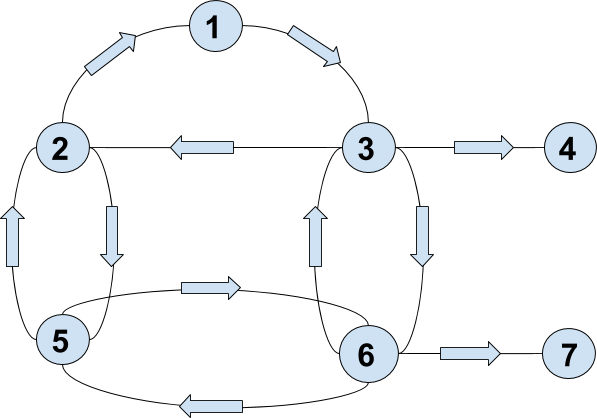
\includegraphics[scale=0.5]{Graf.png}
\end{center}
\noindent
I t.ex. Googles sökalgoritm tänker man sig att sidor med många länkar in eller ut är mer relevanta/viktiga för ett visst ämne/sökfråga.
\begin{Ex}
    Sida \textcircled{3} ovan är mer relevant än t.ex. \textcircled{7}
\end{Ex}

Övergångsmatrisen för grafen ovan:
\[
\mathbf{P} = 
   	\begin{bmatrix}
   		0 & 1/2 & 0 & 0 & 0 & 0 & 0 \\
   		0 & 0 & 1/3 & 0 & 1/2 & 0 & 0 \\
   		1 & 0 & 0 & 0 & 0 & 1/3 & 0 \\
   		0 & 0 & 1/3 & 1 & 0 & 0 & 0 \\
   		0 & 1/2 & 0 & 0 & 0 & 1/3 & 0 \\
   		0 & 0 & 1/3 & 0 & 1/2 & 0 & 0 \\
   		0 & 0 & 0 & 0 & 0 & 1/3 & 1 \\
   	\end{bmatrix}
\]
I en slumpvandring så kommer den stationära fördelningen att beskriva sannolikheten att vara på en viss sida i det långa loppet.
\begin{itemize}
	\item Vi använde markovkedja för att utföra slumpvandring.
	\item Varje markovkedja med reguljär övergångsmatris \textbf{P} har en stationär fördelning. Som är egenvektorn hörande till egenvärdet 1 (det största egenvärdet i \textbf{P}).
	\item \textbf{P} är reguljär om det finns något $\mathbf{P}^k$ där alla element $>0$.
\end{itemize}
I ex. ovan, om man kommit till \textcircled{4} eller \textcircled{7} fastnar man. I slumpvandringen kommer man att få två egenvektorer hörande till egenvärdet 1.\\
I Googles fall justeras \textbf{P} enligt följande:
\begin{itemize}
	\item Om vi hamnat i \textcircled{7} eller \textcircled{4} kan vi välja vilken nod som helst, och ta oss vidare. Kolumn 4 och 7 i \textbf{P} blir $\begin{bmatrix} 1/7 & 1/7 & ... & 1/7 \end{bmatrix}^{T}$
\end{itemize}
Vi får då:
\[
\mathbf{P} = 
   	\begin{bmatrix}
   		0 & 1/2 & 0 & 1/7 & 0 & 0 & 1/7 \\
   		0 & 0 & 1/3 & 1/7 & 1/2 & 0 & 1/7 \\
   		1 & 0 & 0 & 1/7 & 0 & 1/3 & 1/7 \\
   		0 & 0 & 1/3 & 1/7 & 0 & 0 & 1/7 \\
   		0 & 1/2 & 0 & 1/7 & 0 & 1/3 & 1/7 \\
   		0 & 0 & 1/3 & 1/7 & 1/2 & 0 & 1/7 \\
   		0 & 0 & 0 & 1/7 & 0 & 1/3 & 1/7 \\
   	\end{bmatrix}
\]
\begin{itemize}
	\item Även vissa typer av cykler i den underliggande grafen kan göra \textbf{P} icke-reguljär.
\end{itemize}
Vår Google-matris ($\mathbf{G}$) är:
\[
    \mathbf{G} = \overbrace{0.85 \cdot \mathbf{P}}^1 + \overbrace{0.15 [1/n]}^2
\]
\begin{enumerate}
	\item Om man är på viss sida, väljer man att klicka enligt grafen.
	\item Väljer vilken nod som helst i gruppen.
\end{enumerate}
% section _ (end)
\paragraph{-} % (fold)
\label{par:_1}
Hur beräknas egenvektorn till egenvärdet 1.
Vi kan ej lösa:
\[
    (\mathbf{G} - \lambda \cdot \mathbf{I}) \cdot \vec{v}_1 = \emptyset
\]
ty \textbf{G} är för stor.\\
\textbf{Lösning: Potensmetoden}
\begin{gather*}
	\vec{x}_0 = \mbox{standardfördelning} \\
	\vec{x}_{k+1} = \mathbf{G} \cdot \vec{x}_k\\
	k = 0, 1, 2, 3, ...
\end{gather*}
% paragraph _1 (end)
\section{Potensmetoden (power method)} % (fold)
\label{sec:potensmetoden_}
Låt $\lambda_1, \lambda_2, ..., \lambda_n$ vara egenvärden till \textbf{P} och sammanhörande egenvektorer $\vec{v}_1, \vec{v}_2, ..., \vec{v}_n$\\
Om:
\[
    \abs{\lambda_1} > \abs{\lambda_2} \ge \abs{\lambda_3} \ge ... \ge \abs{\lambda_n}
\]
Låt:
\[
    \vec{x} = c_1 \cdot \vec{v}_1 + c_2 \cdot \vec{v}_2 + ... + c_n \cdot \vec{v}_n
\]
Vi har då:
\begin{gather*}
	\mathbf{G}^k \vec{x} = c_1 \cdot \mathbf{G}^k \cdot \vec{v}_1 + ... + c_n \mathbf{G}^k \cdot \vec{v}_n = \\
	c_1 \lambda_1^k \cdot \vec{v}_1 + c_2 \lambda_2^k \cdot \vec{v}_2 + ... + c_n \lambda_n^k \cdot \vec{v}_n
\end{gather*}
Antag $c_1 \neq 0$, dela $(\lambda_1^k)$:
\[
    \frac{1}{\lambda_1^k} \mathbf{G}^k \cdot \vec{x} = c_1 \vec{v}_1 + \Big(\frac{\lambda_2}{\lambda_1}\Big)^k \cdot c_1 \vec{v}_2 + ... + c_n \cdot \Big(\frac{\lambda_n}{\lambda_1}\Big)^k \vec{v}_n
\]
% section potensmetoden_ (end)
\end{document}